\chapter{\textbf{标题}}%第二章
\section[\textnormal{标题}]{\textbf{标题}}

\subsection[\textnormal{标题}]{\textbf{标题}}

可以学学用tikz画图,更加美观,推荐https://www.mathcha.io/editor 画图后导出tikz代码像下面这样引入
注:[htbp]表示图片在该位置附近可以浮动,让计算机自动寻找最佳位置;如果不习惯可以改用[H]来强制固定图片或者表格的位置
\begin{figure}[htbp]
    \centering
    \tikzset{every picture/.style={line width=0.75pt}} %set default line width to 0.75pt        

    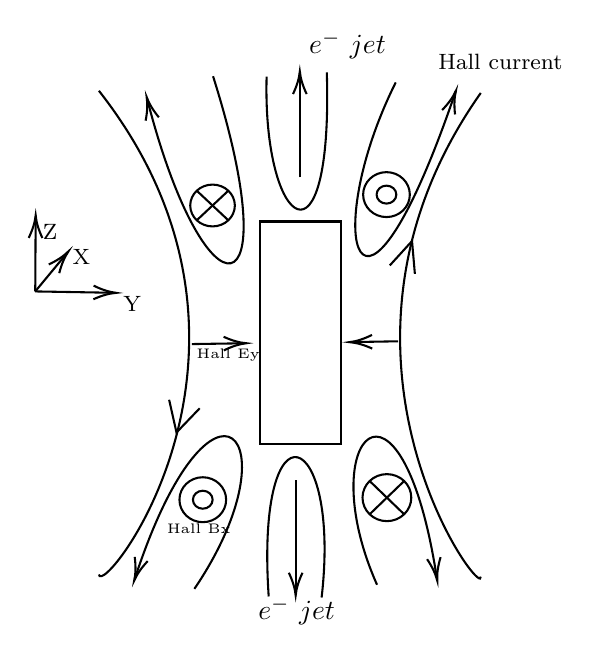
\begin{tikzpicture}[x=0.75pt,y=0.75pt,yscale=-1,xscale=1]
    %uncomment if require: \path (0,338); %set diagram left start at 0, and has height of 338
    
    %Curve Lines [id:da48323297733043824] 
    \draw    (223.87,50.63) .. controls (321.04,174.5) and (225.16,296.27) .. (223.87,283.68) ;
    %Curve Lines [id:da48145401760589657] 
    \draw    (407.85,51.68) .. controls (384.82,84.33) and (373.92,116.7) .. (370.36,146.47) .. controls (360.29,230.6) and (408.81,294.03) .. (407.85,284.73) ;
    %Shape: Rectangle [id:dp7686996309276799] 
    \draw   (301.35,113.62) -- (340.48,113.62) -- (340.48,220.69) -- (301.35,220.69) -- cycle ;
    %Curve Lines [id:da009097792982276864] 
    \draw    (366.87,46.63) .. controls (329.87,120.63) and (348.87,188.63) .. (395.87,50.63) ;
    \draw [shift={(395.87,50.63)}, rotate = 108.81] [color={rgb, 255:red, 0; green, 0; blue, 0 }  ][line width=0.75]    (10.93,-3.29) .. controls (6.95,-1.4) and (3.31,-0.3) .. (0,0) .. controls (3.31,0.3) and (6.95,1.4) .. (10.93,3.29)   ;
    %Curve Lines [id:da7569758360246022] 
    \draw    (278.87,43.63) .. controls (315.68,160.05) and (275.27,163.6) .. (247.29,55.27) ;
    \draw [shift={(246.87,53.63)}, rotate = 75.72] [color={rgb, 255:red, 0; green, 0; blue, 0 }  ][line width=0.75]    (10.93,-3.29) .. controls (6.95,-1.4) and (3.31,-0.3) .. (0,0) .. controls (3.31,0.3) and (6.95,1.4) .. (10.93,3.29)   ;
    %Curve Lines [id:da06071897699960749] 
    \draw    (269.87,290.63) .. controls (319.62,217) and (278.28,173.07) .. (241.42,284.94) ;
    \draw [shift={(240.87,286.63)}, rotate = 287.98] [color={rgb, 255:red, 0; green, 0; blue, 0 }  ][line width=0.75]    (10.93,-3.29) .. controls (6.95,-1.4) and (3.31,-0.3) .. (0,0) .. controls (3.31,0.3) and (6.95,1.4) .. (10.93,3.29)   ;
    %Curve Lines [id:da7035242269674511] 
    \draw    (357.87,288.63) .. controls (326.03,216.99) and (369.43,174.06) .. (386.61,284.95) ;
    \draw [shift={(386.87,286.63)}, rotate = 261.44] [color={rgb, 255:red, 0; green, 0; blue, 0 }  ][line width=0.75]    (10.93,-3.29) .. controls (6.95,-1.4) and (3.31,-0.3) .. (0,0) .. controls (3.31,0.3) and (6.95,1.4) .. (10.93,3.29)   ;
    %Flowchart: Summing Junction [id:dp4313333309183207] 
    \draw   (267.87,105.91) .. controls (267.87,100.34) and (272.68,95.83) .. (278.62,95.83) .. controls (284.55,95.83) and (289.37,100.34) .. (289.37,105.91) .. controls (289.37,111.47) and (284.55,115.98) .. (278.62,115.98) .. controls (272.68,115.98) and (267.87,111.47) .. (267.87,105.91) -- cycle ; \draw   (271.02,98.78) -- (286.22,113.03) ; \draw   (286.22,98.78) -- (271.02,113.03) ;
    %Flowchart: Summing Junction [id:dp5244689001643144] 
    \draw   (350.87,246.66) .. controls (350.87,240.4) and (356.13,235.33) .. (362.62,235.33) .. controls (369.11,235.33) and (374.37,240.4) .. (374.37,246.66) .. controls (374.37,252.91) and (369.11,257.98) .. (362.62,257.98) .. controls (356.13,257.98) and (350.87,252.91) .. (350.87,246.66) -- cycle ; \draw   (354.31,238.65) -- (370.93,254.67) ; \draw   (370.93,238.65) -- (354.31,254.67) ;
    %Shape: Donut [id:dp24273032973492104] 
    \draw   (357.66,100.66) .. controls (357.66,98.27) and (359.79,96.33) .. (362.42,96.33) .. controls (365.04,96.33) and (367.17,98.27) .. (367.17,100.66) .. controls (367.17,103.05) and (365.04,104.99) .. (362.42,104.99) .. controls (359.79,104.99) and (357.66,103.05) .. (357.66,100.66)(351.17,100.66) .. controls (351.17,94.68) and (356.2,89.83) .. (362.42,89.83) .. controls (368.63,89.83) and (373.67,94.68) .. (373.67,100.66) .. controls (373.67,106.64) and (368.63,111.48) .. (362.42,111.48) .. controls (356.2,111.48) and (351.17,106.64) .. (351.17,100.66) ;
    %Shape: Donut [id:dp5018283498511262] 
    \draw   (269.16,247.66) .. controls (269.16,245.27) and (271.29,243.33) .. (273.92,243.33) .. controls (276.54,243.33) and (278.67,245.27) .. (278.67,247.66) .. controls (278.67,250.05) and (276.54,251.99) .. (273.92,251.99) .. controls (271.29,251.99) and (269.16,250.05) .. (269.16,247.66)(262.67,247.66) .. controls (262.67,241.68) and (267.7,236.83) .. (273.92,236.83) .. controls (280.13,236.83) and (285.17,241.68) .. (285.17,247.66) .. controls (285.17,253.64) and (280.13,258.48) .. (273.92,258.48) .. controls (267.7,258.48) and (262.67,253.64) .. (262.67,247.66) ;
    %Straight Lines [id:da8405097778514081] 
    \draw    (318.67,238.33) -- (318.67,291.78) ;
    \draw [shift={(318.67,293.78)}, rotate = 270] [color={rgb, 255:red, 0; green, 0; blue, 0 }  ][line width=0.75]    (10.93,-3.29) .. controls (6.95,-1.4) and (3.31,-0.3) .. (0,0) .. controls (3.31,0.3) and (6.95,1.4) .. (10.93,3.29)   ;
    %Curve Lines [id:da1273324589984952] 
    \draw    (305.67,294.28) .. controls (299.17,197.28) and (340.67,212.28) .. (331.17,294.78) ;
    %Straight Lines [id:da5675650016597387] 
    \draw    (320.67,92.38) -- (320.67,43.28) ;
    \draw [shift={(320.67,41.28)}, rotate = 90] [color={rgb, 255:red, 0; green, 0; blue, 0 }  ][line width=0.75]    (10.93,-3.29) .. controls (6.95,-1.4) and (3.31,-0.3) .. (0,0) .. controls (3.31,0.3) and (6.95,1.4) .. (10.93,3.29)   ;
    %Curve Lines [id:da8039128203052084] 
    \draw    (304.67,43.78) .. controls (302.67,117.28) and (336.67,141.28) .. (333.67,41.78) ;
    %Straight Lines [id:da4541491512880813] 
    \draw    (268.67,172.67) -- (292.93,172.3) ;
    \draw [shift={(294.93,172.27)}, rotate = 179.13] [color={rgb, 255:red, 0; green, 0; blue, 0 }  ][line width=0.75]    (10.93,-3.29) .. controls (6.95,-1.4) and (3.31,-0.3) .. (0,0) .. controls (3.31,0.3) and (6.95,1.4) .. (10.93,3.29)   ;
    %Straight Lines [id:da7265038531434131] 
    \draw    (368,171.33) -- (346.57,171.7) ;
    \draw [shift={(344.57,171.74)}, rotate = 359.02] [color={rgb, 255:red, 0; green, 0; blue, 0 }  ][line width=0.75]    (10.93,-3.29) .. controls (6.95,-1.4) and (3.31,-0.3) .. (0,0) .. controls (3.31,0.3) and (6.95,1.4) .. (10.93,3.29)   ;
    %Straight Lines [id:da49539526071555806] 
    \draw    (193.2,147.3) -- (230.2,147.95) ;
    \draw [shift={(232.2,147.99)}, rotate = 181.01] [color={rgb, 255:red, 0; green, 0; blue, 0 }  ][line width=0.75]    (10.93,-3.29) .. controls (6.95,-1.4) and (3.31,-0.3) .. (0,0) .. controls (3.31,0.3) and (6.95,1.4) .. (10.93,3.29)   ;
    %Straight Lines [id:da14093049137857494] 
    \draw    (193.2,147.3) -- (193.39,112.6) ;
    \draw [shift={(193.4,110.6)}, rotate = 90.31] [color={rgb, 255:red, 0; green, 0; blue, 0 }  ][line width=0.75]    (10.93,-3.29) .. controls (6.95,-1.4) and (3.31,-0.3) .. (0,0) .. controls (3.31,0.3) and (6.95,1.4) .. (10.93,3.29)   ;
    %Straight Lines [id:da8298958012348723] 
    \draw    (193.2,147.3) -- (207.92,129.53) ;
    \draw [shift={(209.2,127.99)}, rotate = 129.64] [color={rgb, 255:red, 0; green, 0; blue, 0 }  ][line width=0.75]    (10.93,-3.29) .. controls (6.95,-1.4) and (3.31,-0.3) .. (0,0) .. controls (3.31,0.3) and (6.95,1.4) .. (10.93,3.29)   ;
    \draw   (272.45,203.59) -- (261.25,215.26) -- (257.7,199.49) ;
    \draw   (364.03,134.77) -- (374.73,123.03) -- (376.1,138.85) ;
    
    % Text Node
    \draw (323.67,20.73) node [anchor=north west][inner sep=0.75pt]    {$e^{-} \ jet$};
    % Text Node
    \draw (299.17,293.37) node [anchor=north west][inner sep=0.75pt]    {$e^{-} \ jet$};
    % Text Node
    \draw (385.9,31.48) node [anchor=north west][inner sep=0.75pt]   [align=left] {{\footnotesize Hall current}};
    % Text Node
    \draw (269.49,173.34) node [anchor=north west][inner sep=0.75pt]   [align=left] {{\tiny Hall Ey}};
    % Text Node
    \draw (209.72,125.47) node [anchor=north west][inner sep=0.75pt]  [rotate=-0.15] [align=left] {{\footnotesize X}};
    % Text Node
    \draw (234.2,147.99) node [anchor=north west][inner sep=0.75pt]   [align=left] {{\footnotesize Y}};
    % Text Node
    \draw (195.4,113.6) node [anchor=north west][inner sep=0.75pt]   [align=left] {{\footnotesize Z}};
    % Text Node
    \draw (255.2,257.84) node [anchor=north west][inner sep=0.75pt]   [align=left] {{\tiny Hall Bx}};
    
    
    \end{tikzpicture}
    \caption{Hall重联截面示意图}
\label{reconnect_cross_section}

\end{figure}

\subsubsection{\textbf{标题}}
